\documentclass[a4paper,12pt]{article}
\usepackage{fontspec}
\usepackage{xeCJK}
%\usepackage{helvet}
%\setCJKmainfont{SimSun}
\setmainfont{Times New Roman}
%\setmainfont{helvet}
\usepackage[english]{babel}
%\usepackage[utf8]{inputenc}

%\usepackage[T1]{fontenc}
\usepackage{amsmath}
\usepackage{amsthm}
\usepackage{amsfonts}
\usepackage{amssymb}
\usepackage{graphicx}
\usepackage{hyperref}
\usepackage{enumitem}
\usepackage{textcomp}
\usepackage{float}
\usepackage{booktabs}
%\usepackage{CJKutf8}

\usepackage[colorinlistoftodos]{todonotes}
\usepackage[left=1.50cm, right=1.50cm, top=1.20cm]{geometry}
\linespread{1.5}
\usepackage{algorithm}
\usepackage{algpseudocode}

\usepackage{tikz}
\usepackage[tikz]{mdframed}
\usetikzlibrary{matrix, positioning, fit, arrows, calc, intersections, shapes, shadings, patterns, decorations.markings, chains, scopes}

\usepackage{upquote}
\usepackage{listings}
\lstset{upquote=true}
\lstdefinestyle{customc}{
  belowcaptionskip=1\baselineskip,
  breaklines=true,
  frame=L,
  xleftmargin=\parindent,
  language=C++,
  tabsize=2,
  showstringspaces=false,
  basicstyle=\small\ttfamily,
  keywordstyle=\bfseries\color{green!40!black},
  commentstyle=\itshape\color{purple!40!black},
  identifierstyle=\color{blue},
  stringstyle=\color{orange},
}
\mdfdefinestyle{mymdf}{leftmargin=1cm,rightmargin=2cm,%
innerleftmargin=1cm,innerrightmargin=1cm,roundcorner=10pt,backgroundcolor=lg}
\definecolor{lg}{RGB}{247,249,250}
\title{Algorithm Problem Set \\ \large No. 1001 --- 1099}
%\title{Functional Programming In C++}
\author{SS}
\date{April 2019}

\begin{document}
\def\bottom#1#2{\hbox{\vbox to #1{\vfill\hbox{#2}}}}
%\fontfamily{phv}\selectfont
\renewcommand{\thelstlisting}{\thesection.\arabic{lstlisting}}
\sloppy
\maketitle
\section{1025 --- Divisor Game}
Alice and Bob take turns playing a game, with Alice starting first.
\par
Initially, there is a number $ N $ on the chalkboard.  On each player's turn, that player makes a \textit{move} consisting of:
\begin{itemize}
\item Choosing any $ x $ with $ 0 < x < N $ and $ N \bmod x = 0 $.
\item Replacing the number $ N $ on the chalkboard with $ N - x $.
\end{itemize}
\par
Also, if a player cannot make a move, they lose the game.
\par
Return \texttt{true} if and only if Alice wins the game, assuming both players play optimally.

 
\paragraph{Example 1:}

\begin{flushleft}
\textbf{Input}: 2
\\
\textbf{Output}: \texttt{true}
\\
\textbf{Explanation}: Alice chooses 1, and Bob has no more moves.
\end{flushleft}

\paragraph{Example 2:}

\begin{flushleft}
\textbf{Input}: 3
\\
\textbf{Output}: \texttt{false}
\\
\textbf{Explanation}: Alice chooses 1, Bob chooses 1, and Alice has no more moves.
\end{flushleft}
 

\paragraph{Note:}
\begin{itemize}
\item $ 1 \leq N \leq 1000 $
\end{itemize}

\subsection{Mathematical Induction}
\begin{itemize}
\item 如果 $N$是奇数,Alice 会输
\item 否则,当$N$是偶数时,Alice会赢。
\end{itemize}
\section{1026 --- Maximum Difference Between Node and Ancestor}
Given the root of a binary tree, find the maximum value $ V $ for which there exists different nodes $ A $ and $ B $ where $V = |V_A - V_B|$ and $A$ is an ancestor of $B$.
\par
(A node $ A $ is an ancestor of $ B $ if either: any child of $ A $ is equal to $ B $, or any child of $ A $ is an ancestor of $ B $.)
\paragraph{Example 1:}
\begin{flushleft}
\begin{figure}[H]
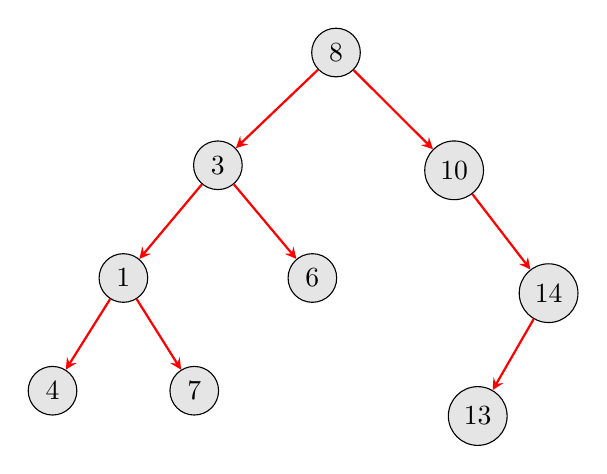
\begin{tikzpicture}
[my/.style={draw, circle, fill=gray!20, minimum size=5mm}]
\node[my] (1) at (0,0) {8};
\node[my] (2) [below=8mm of 1, xshift=-15mm] {3};
\node[my] (3) [below=8mm of 1, xshift=15mm] {10};
\node[my] (4) [below=8mm of 2, xshift=-12mm] {1};
\node[my] (5) [below=8mm of 2, xshift=12mm] {6};
\node[my] (6) [below=8mm of 3, xshift=12mm] {14};
\node[my] (7) [below=8mm of 4, xshift=-9mm] {4};
\node[my] (8) [below=8mm of 4, xshift=9mm] {7};
\node[my] (9) [below=8mm of 6, xshift=-9mm] {13};
\draw[thick,red,>=stealth,->] (1) -- (2);
\draw[thick,red,>=stealth,->] (1) -- (3);
\draw[thick,red,>=stealth,->] (2) -- (4);
\draw[thick,red,>=stealth,->] (2) -- (5);
\draw[thick,red,>=stealth,->] (3) -- (6);
\draw[thick,red,>=stealth,->] (4) -- (7);
\draw[thick,red,>=stealth,->] (4) -- (8);
\draw[thick,red,>=stealth,->] (6) -- (9);
\end{tikzpicture}
\end{figure}
\textbf{Input}: $[8,3,10,1,6,\varnothing,14,\varnothing,\varnothing,4,7,13]$
\\
\textbf{Output}: 7
\\
\textbf{Explanation}: 
\\
We have various ancestor-node differences, some of which are given below:
$\lvert8 - 3\rvert = 5$
\\
$\lvert 3 - 7\rvert = 4$
\\
$\lvert 8 - 1\rvert = 7$
\\
$\lvert 10 - 13\rvert| = 3$
\\
Among all possible differences, the maximum value of 7 is obtained by $\lvert8 - 1\rvert = 7$.
 \end{flushleft}
 
\paragraph{Note:}

\begin{itemize}
\item The number of nodes in the tree is between 2 and 5000.
\item Each node will have value between 0 and 100000.
\end{itemize}

\setcounter{lstlisting}{0}
\begin{lstlisting}[style=customc, caption={TODO}]
int maxAncestorDiff( TreeNode* root )
{
}
\end{lstlisting}
\section{1027 --- Longest Arithmetic Sequence}
Given an array $ A $ of integers, return the length of the longest arithmetic subsequence in $ A $.
\par
Recall that a subsequence of $ A $ is a list $ A[i_1] $, $ A[i_2] $, $ \ldots $, $ A[i_k] $ with $0 <= i_1 < i_2 < \ldots < i_k \leq |A| - 1$, and that a sequence B is arithmetic if $B[i+1] - B[i]$ are all the same value (for $0 \leq i < |B| - 1$).

\paragraph{Example 1:}

\begin{flushleft}
\textbf{Input}: $[3,6,9,12]$
\\
\textbf{Output}: 4
\\
\textbf{Explanation}:
\\ 
The whole array is an arithmetic sequence with steps of length = 3.
\end{flushleft}


\paragraph{Example 2:}

\begin{flushleft}
\textbf{Input}: $[9,4,7,2,10]$
\\
\textbf{Output}: 3
\\
\textbf{Explanation}:
\\
The longest arithmetic subsequence is $[4,7,10]$.
\end{flushleft}

\paragraph{Example 3:}

\begin{flushleft}
\textbf{Input}: $[20,1,15,3,10,5,8]$
\\
\textbf{Output}: 4
\\
\textbf{Explanation}: 
\\
The longest arithmetic subsequence is $[20,15,10,5]$.
\end{flushleft}

\paragraph{Note:}

\begin{itemize}
\item $2 \leq |A| \leq 2000$
\item $0 \leq A[i] \leq 10000$
\end{itemize}

\subsection{Dynamic Programming}
\begin{itemize}
\item 用一个array $F$作为Dynamic Programming的递推数组。其中每个元素都是一个hash map,其key是等差数列的差值,而value则是这个等差数列的长度
\item 对于当前index $i$,从0到$i-1$的每一个index $j$,根据$A[i]$与$A[j]$之间的差值,找到以$A[i]$为end的所形成的所有可能的等差数列,并记录相应的长度。
\end{itemize}

\setcounter{lstlisting}{0}
\begin{lstlisting}[style=customc, caption={Dynamic Progamming}]
int longestArithSeqLength( vector<int>& A )
{
    //DP array
    vector<unordered_map<int, int>> F( A.size() );

    int ans = 1;

    for( size_t i = 1; i < A.size(); ++i )
    {
        for( size_t j = 0; j < i; ++j )
        {
            int diff = A[i] - A[j];

            int l = 1;
            //get the sequence end at A[j] with diff
            auto it = F[j].find( diff );
            if( it != F[j].end() )
            {
                l = it->second + 1;
            }

            auto it_cur = F[i].find( diff );

            if( it_cur == F[i].end() )
            {
                F[i].emplace( diff, l );
            }
            else
            {
                //to account for duplicate number
                //we should choose the maximum length so far
                it_cur->second = ( max )( it_cur->second, l );
            }

            ans = ( max )( ans, l );
        }
    }

    //The sequence length need to account for
    //the start number, so add 1 to the answer
    return ans + 1;

}
\end{lstlisting}
\section{1028 --- Recover a Tree From Preorder Traversal}
We run a preorder depth first search on the root of a binary tree.
\par
At each node in this traversal, we output $ D $ dashes (where $ D $ is the depth of this node), then we output the value of this node.  (If the depth of a node is $ D $, the depth of its immediate child is $ D+1 $.  The depth of the root node is 0.)
\par
If a node has only one child, that child is guaranteed to be the left child.
\par
Given the output $ S $ of this traversal, recover the tree and return its root.
\paragraph{Example 1:}
\begin{flushleft}
\begin{figure}[H]
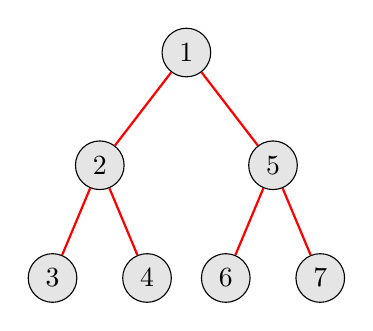
\begin{tikzpicture}
[my/.style={draw, circle, fill=gray!20, minimum size=5mm}]
\node[my] (1) at (0,0) {1};
\node[my] (2) [below=8mm of 1, xshift=-11mm] {2};
\node[my] (3) [below=8mm of 1, xshift=11mm] {5};
\node[my] (4) [below=8mm of 2, xshift=-6mm] {3};
\node[my] (5) [below=8mm of 2, xshift=6mm] {4};
\node[my] (6) [below=8mm of 3, xshift=-6mm] {6};
\node[my] (7) [below=8mm of 3, xshift=6mm] {7};
\draw[thick,red] (1) -- (2);
\draw[thick,red] (1) -- (3);
\draw[thick,red] (2) -- (4);
\draw[thick,red] (2) -- (5);
\draw[thick,red] (3) -- (6);
\draw[thick,red] (3) -- (7);
\end{tikzpicture}
\end{figure}
\textbf{Input}: $1D2DD3DD4D5DD6DD7$ ($ D $ is a dash)
\\
\textbf{Output}: $[1,2,5,3,4,6,7]$
\end{flushleft}

\paragraph{Example 2:}
\begin{flushleft}
\begin{figure}[H]
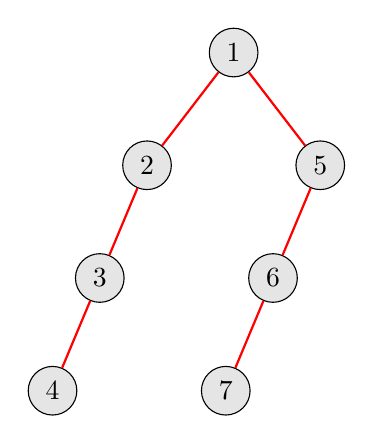
\begin{tikzpicture}
[my/.style={draw, circle, fill=gray!20, minimum size=5mm}]
\node[my] (1) at (0,0) {1};
\node[my] (2) [below=8mm of 1, xshift=-11mm] {2};
\node[my] (3) [below=8mm of 1, xshift=11mm] {5};
\node[my] (4) [below=8mm of 2, xshift=-6mm] {3};
\node[my] (5) [below=8mm of 4, xshift=-6mm] {4};
\node[my] (6) [below=8mm of 3, xshift=-6mm] {6};
\node[my] (7) [below=8mm of 6, xshift=-6mm] {7};
\draw[thick,red] (1) -- (2);
\draw[thick,red] (1) -- (3);
\draw[thick,red] (2) -- (4);
\draw[thick,red] (4) -- (5);
\draw[thick,red] (3) -- (6);
\draw[thick,red] (6) -- (7);
\end{tikzpicture}
\end{figure}
\textbf{Input}: $1D2DD3DDD4D5DD6DDD7$ ($ D $ is a dash)
\\
\textbf{Output}: $[1,2,5,3,\varnothing,6,\varnothing,4,\varnothing,7]$
\end{flushleft}

\paragraph{Example 3:}
\begin{flushleft}
\begin{figure}[H]
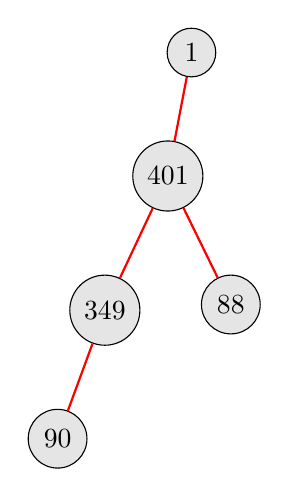
\begin{tikzpicture}
[my/.style={draw, circle, fill=gray!20, minimum size=5mm}]
\node[my] (1) at (0,0) {1};
\node[my] (2) [below=8mm of 1, xshift=-3mm] {401};
\node[my] (3) [below=8mm of 2, xshift=-8mm] {349};
\node[my] (4) [below=8mm of 2, xshift=8mm] {88};
\node[my] (5) [below=8mm of 3, xshift=-6mm] {90};
\draw[thick,red] (1) -- (2);
\draw[thick,red] (2) -- (3);
\draw[thick,red] (2) -- (4);
\draw[thick,red] (3) -- (5);
\end{tikzpicture}
\end{figure}
\textbf{Input}: $1D401DD349DDD90DD88$ ($ D $ is a dash)
\\
\textbf{Output}: $[1,401,\varnothing,349,88,90]$
\end{flushleft}

\paragraph{Note:}

\begin{itemize}
\item The number of nodes in the original tree is between 1 and 1000. 
\item Each node will have a value between 1 and $ 10^9 $.
\end{itemize}

\subsection{Hash Map}
\begin{itemize}
\item 创建一个hash map $M$,其key为level的number,而value为数组,存放当前level所有create出的tree node以及该tree node对应的parent node。
\item 遍历原数组,对于每个数字,创建相应的Tree Node。然后根据相应的level,找到上一层即level-1对应的parent。由于preorder的特性,以及我们设计的数据结构的特点,上一层的level对应的数组的倒数第二个node即为当前create出的node的parent。(最后一个node是这个parent的parent node)。
\item 最后从level = 1开始,将每个node与其parent node相连,先检查parent node的left child是否为null,如果是,将当前node设置为parent node的left child,否则设置为right child。(题目中说明了如果只有一个child,必定是left child)。
\end{itemize}

\setcounter{lstlisting}{0}
\begin{lstlisting}[style=customc, caption={Hash Map}]
TreeNode* recoverFromPreorder( string S )
{
    if( S.empty() )
    {
        return nullptr;
    }

    //add dash to let state change can
    //happen at the end of S
    S.push_back( '-' );

    //the hash map to
    //store each level's node and its parent
    unordered_map<int, vector<TreeNode*>> m_levels;

    int level = 0;
    int x = 0;

    int max_level = 0;
    TreeNode* parent = nullptr;

    int state = 1; //1=digit,2=dash

    for( auto c : S )
    {
        if( c != '-' )
        {
            if( state == 2 )
            {
                //update maximum level so far
                max_level = ( max )( level, max_level );
                //change state to 1
                //to indicate we are collecting numbers
                state = 1;
            }

            x = x * 10 + ( c - '0' );
        }
        else
        {
            if( state == 1 )
            {
                auto node = new TreeNode( x );

                if( level > 0 )
                {
                    //get node's parent
                    auto it = m_levels.find( level - 1 );
                    auto sz = it->second.size();
                    //the last element if the parent of parent
                    //the one to the last element is the parent
                    parent = it->second[sz - 2];
                }

                auto it = m_levels.find( level );
                if( it == m_levels.end() )
                {
                    //we put node and its parent along each other
                    m_levels.emplace( level, initializer_list<TreeNode*> {node, parent} ).first;
                }
                else
                {
                    it->second.emplace_back( node );
                    it->second.emplace_back( parent );
                }


                //reset level and x
                level = 0;
                x = 0;

                //change state to 2
                //to indicate we are counting dashes
                state = 2;
            }

            ++level;
        }
    }

    //now, we link the nodes to its parent
    for( int level = 1; level <= max_level; ++level )
    {
        auto& nodes = m_levels[level];

        for( size_t i = 0; i < nodes.size(); i += 2 )
        {
            if( !nodes[i + 1]->left )
            {
                //left child has not been set
                //set to left child
                nodes[i + 1]->left = nodes[i];
            }
            else
            {
                //left child has been set
                //set to right child
                nodes[i + 1]->right = nodes[i];
            }
        }
    }

    //root is at the level 0
    return m_levels[0][0];
}
\end{lstlisting}


\subsection{Stack}
\begin{itemize}
\item 创建一个stack,其中存放create出来的tree node。
\item 同样是从$S$中获取node的value和对应的level。然后根据value create一个新的node。
\item 如果当前level比stack的size还要小,说明stack中包含了和当前node以及其child nodes相同level的nodes,将这些 nodes 从 stack 中移除, 直到stack的size等于当前level。
\item 如果这时候stack不为空,那么这时候stack的top元素就是当前node的parent。(简单的推理: 当stack的size为1时,就只有root node。而root node的level为零。) 根据这个parent的左右子节点是否为null,来设定当前node为left child还是right child。
\item 最后如果$S$的size不为1,需要将多余的元素弹出,因为最终需要的是$S$最底下的root node。
\end{itemize}

\setcounter{lstlisting}{0}
\begin{lstlisting}[style=customc, caption={Stack}]
TreeNode* recoverFromPreorder( string S )
{
    if( S.empty() )
    {
        return nullptr;
    }

    S.push_back( '-' );

    stack<TreeNode*> stk;

    size_t level = 0;
    int x = 0;

    size_t max_level = 0;
    TreeNode* parent = nullptr;

    int state = 1; //1=digit,2=dash

    for( auto c : S )
    {
        if( c != '-' )
        {
            if( state == 2 )
            {
                max_level = ( max )( level, max_level );
                state = 1;
            }

            x = x * 10 + ( c - '0' );
        }
        else
        {
            if( state == 1 )
            {
                auto node = new TreeNode( x );

                //find the parent of node
                while( !stk.empty() && stk.size() > level )
                {
                    stk.pop();
                }

                if( !stk.empty() )
                {
                    //stk.top() is the parent of node
                    if( !stk.top()->left )
                    {
                        stk.top()->left = node;
                    }
                    else
                    {
                        stk.top()->right = node;
                    }

                }

                //push node into the stack
                stk.push( node );


                level = 0;
                x = 0;

                state = 2;
            }

            ++level;
        }
    }

    //we need to pop unnecessary nodes
    //to get root node
    while( stk.size() > 1 )
    {
        stk.pop();
    }

    return stk.top();
}
\end{lstlisting}
\section{1032 --- Stream of Characters}
Implement the \texttt{StreamChecker} class as follows:

\begin{lstlisting}[style=customc]
StreamChecker(words): //Constructor, init the data structure with the given words.
query(letter): //returns true if and only if for some k >= 1, the last k characters queried (in order from oldest to newest, including this letter just queried) spell one of the words in the given list.
\end{lstlisting}
 

\paragraph{Example:}

\begin{lstlisting}[style=customc]
StreamChecker streamChecker = new StreamChecker(["cd","f","kl"]); // init the dictionary.
streamChecker.query('a'); // return false
streamChecker.query('b'); // return false
streamChecker.query('c'); // return false
streamChecker.query('d'); // return true, because 'cd' is in the wordlist
streamChecker.query('e'); // return false
streamChecker.query('f'); // return true, because 'f' is in the wordlist
streamChecker.query('g'); // return false
streamChecker.query('h'); // return false
streamChecker.query('i'); // return false
streamChecker.query('j'); // return false
streamChecker.query('k'); // return false
streamChecker.query('l'); // return true, because 'kl' is in the wordlist
\end{lstlisting}
 

\paragraph{Note:}

\begin{itemize}
\item $1 \leq L \leq 2000$. $L$ is the length of input words array
\item $1 \leq l_i \leq 2000$ $l_i$ is the length of word at index $i$
\item \texttt{Words} will only consist of lowercase English letters.
\item \texttt{Queries} will only consist of lowercase English letters.
\item The number of queries is at most 40000.
\end{itemize}

\end{document}